\documentclass{kththesis}

\usepackage{blindtext} % This is just to get some nonsense text in this template, can be safely removed
\usepackage[linesnumbered,ruled]{algorithm2e}
\usepackage{amsmath}
\usepackage{booktabs}
\usepackage{biblatex}
\usepackage{chngpage}
\usepackage{csquotes} % Recommended by biblatex
\usepackage{hyperref}
\usepackage{graphicx}
\usepackage{mwe}
\usepackage{multirow}
\usepackage[parfill]{parskip}
\usepackage{subcaption}

\addbibresource{references.bib} % The file containing our references, in BibTeX format


% --- TITLE & FRONT PAGE ---

\title{Feature Selection Methods for Classification of Breast Cancer}
\alttitle{Attributurvalsmetoder för klassificering av bröstcancer }
\author{Niklas Lindqvist\newline Thony Price}
\email{nlinq@kth.se\newline thonyp@kth.se}
\supervisor{Pawel Herman}
\examiner{örjan Ekeberg}
\programme{Degree Project in Computer Science}
\school{School of Computer Science and Communication}
\date{\today}


\begin{document}
% Frontmatter includes the titlepage, abstracts and table-of-contents
\frontmatter
\titlepage


% --- ABSTRACT ENGLISH ---

\begin{abstract}

  Breast cancer is the leading cause of cancer deaths among women today but computer aided diagnosis has proved efficient in assisting medical experts to set an early diagnosis improving the chance of recovery. Computer aided diagnostics utilises machine learning to make a prediction whether a patient has a benign or malignant cancer. In the process a patients data is put into machine learning algorithms and a classification is made. Applying feature selection mean algorithms can be fed data with lower dimensionality and produce a more accurate result. We've found classifiers from different disciplines of machine learning all see the benefit of a higher classification accuracy when using feature selection.

\end{abstract}


% --- ABSTRACT SWEDISH ---

\begin{otherlanguage}{swedish}
  \begin{abstract}

  Brostcancer ar idag den ledande cancerformen som orsakar for tidig dod hos kvinnor. Datordriven diagnostisering har visat sig effektiv i att assistera medicinska experter med att satta en tidig diagnos for cancers och darmed oka chanserna for tillfrisknande hos patienten. Datordriven diagnostisering anvander sig av maskininlarningsmetoder for att gora en prediktion huruvida en patient har god eller elakartad cancer. I denna processes anvands en patients data av maskininlarningsalgoritmen och en klassificering kan goras. Applikationen av attributurvalsmetoder innebar att algoritmen kan anvanda sig av data med farre dimensioner och producera ett mer traffsakert resultat. Vi fann att klassificerare fran olika dicipliner av maskininlarning alla visade fordelen med hogre klassificeringstraffsakerhet nar attributurvalsmetoder anvandes.

  \textit{Fix swedish symbols for ao ae oe here...}

  \end{abstract}

\end{otherlanguage}


\tableofcontents
% Mainmatter is where the actual contents of the thesis goes
\mainmatter


% --- CONTENT ---

% --- 1. INTRODUCTION CHAPTER ---
\chapter{Introduction}

Breast cancer is a disease of major concern and is the leading cause of cancer deaths among women \parencite{althuis2005}. At present there are no effective ways to prevent breast cancer. However, efficient diagnosis in an early stage can increase the chance of full recovery. This makes early detection and diagnosis an important issue where currently mammography screenings is the primary imaging modality for early detection of breast cancer \parencite{tabar2001}.

Hospitals today collect data to do monitoring and some of this data, such as mammography screenings can be collected and shared in information systems. The data can be used by medical personnel to increase their understanding of different diseases. It can also be used in computer aided diagnostics (CAD) where machine learning algorithms enable tools for intelligent data analysis. CAD makes use of machine learning techniques that learn a hypothesis, a statistical prediction about a patient's diagnosis from a large set of previously diagnosed examples.  The overarching purpose is to assist medical experts in more efficient and accurate diagnostics \parencite{li2007}. Machine learning algorithms is a well studied field within medical diagnosis and well suited for analyzing medical data, especially within small specialized diagnostic problems such as breast cancer \parencite{kononenko2001}.

Multiple studies of CAD on breast cancer have been conducted, primarily focusing on classifying mammography data of tumors as malignant or not, such those of \textcite{ramos2012} and \textcite{akay2009}. The act of feature selection, removing redundant or irrelevant features from a dataset, can provide classifiers to be faster, more cost-effective and accurate. With feature selection the understandability can be improved which is a clear benefit when it comes to medical decisions \parencite{karabulut2012}. It is also explicitly mentioned as a topic in need of more research in studies made on breast cancer diagnostics \parencite{akin2011}.


\section{Research Question}

In our thesis we will study the impact of four feature selection methods on the classification rate of malignant breast cancer by four different machine learning methods. We aim to answer the following:

\begin{itemize}
  \item Does the feature selection improve the accuracy of classification compared to using all features?
  \item Is the effect of feature selection dependent on the classification method?
\end{itemize}

Our hypothesis is that overall the feature selection will improve the classification rate of the machine learning methods used in the context of breast cancer classification. This hypothesis is based on previous research reported by \textcite{karabulut2012}, where it was found that classification accuracy on 15 different datasets of medical and non-medical data was increased by the use of filtering methods for feature selection.

Our research differs from the work presented in \parencite{karabulut2012} in the amount of datasets used and number of classification methods. In our project we will put more emphasis on breast cancer using only datasets of that type. The previous work only investigated feature selection methods by filtering which we will extend by implementing wrapper methods. Lastly, the research scope in this thesis includes a study of the effect of different feature selection methods on Support Vector Machines (SVMs), which was not included in \parencite{karabulut2012}.


\section{Approach}

Trials will be conducted with feature selection by using both wrapper methods and feature selection filter methods. The result of the feature selection methods will be used with different classifiers to evaluate their performance. To broaden the base for comparison we will use several classifiers, Decision Tree (DT) a logic based algorithms, Artificial Neural Network (ANN) a perceptron-based technique, Naïve Bayes (NB) a statistical learning algorithms and Support Vector Machines (SVM) \parencite{wallace2007}. These classifiers are commonly used in CAD and thus relevant to study \parencite{ramos2012}, \parencite{akay2009}, \parencite{li2007}. Feature selection (FS) methods and classifiers included in this report are denoted in table \ref{table:methods}.

\begin{table}[ht]
\begin{center}
\begin{tabular}{ l | l }
\multicolumn{2}{ c }{\textbf{Included classifiers and FS-methods}} \\
\hline
\multirow{4}{*}{Classifiers}
 & Artificial Neural Network (ANN) \\
 & Decision Tree (DT) \\
 & Naïve Bayes (NB) \\
 & Support Vector Machine (SVM) \\ \hline
\multirow{2}{*}{FS by Wrapping}
 & Sequential Backward FS (SBS) \\
 & Sequential Forward FS (SFS) \\ \hline
\multirow{2}{*}{FS by Filtering}
 & Chi-square (Chi2) \\
 & Entropy \\
\hline
\end{tabular}
\caption[]
{\small All classifiers and feature selection methods included in this paper. Each classifier will be tested with each FS-method yielding 16 distinct combinations.}
\label{table:methods}
\end{center}
\end{table}


A comparison between the classification rate of the machine learning methods without using any feature selection, and classification rate when using feature selection will be conducted. The comparison may then establish the importance of feature selection in different machine learning approaches when classifying breast cancer. The evaluation of impact by FS will be measured by computing the ratio between best accuracy achieved with and without using feature selection. Several datasets with different types of features will be used for evaluation. Details on the datasets will be presented in section \ref{sec:Datasets}. The reason for using multiple datasets is to strengthen the basis for statistical evaluation and possibility conclude a more generalized result.


\section{Scope}

The scope of this thesis is limited by the amount of datasets, classifiers and FS-methods included. Having four of each, the aim is to conclude a result that generalize well. However, it must be considered these are a small selection of all the available possibilities. The data represents a few of the possible ways to collect data when making breast cancer diagnostics. There are many more classifiers and each can be tuned into countless of configurations. Regarding the feature selection methods we evaluate two filter methods and two wrapper methods, it exists many more and also embedded methods which is not included in out thesis.

These limitations results in constraining our scope to the classifiers and FS-methods presented in table \ref{table:methods} and the datasets described in \ref{sec:Datasets}.


% --- 2. BACKGROUND CHAPTER ---
\chapter{Background}


\section{Computer Aided Diagnostics}

Machine learning techniques have been successfully applied to computer-aided diagnosis where it by a computerized procedure provides a second objective opinion for the assistance of medical image interpretation and diagnosis \parencite{li2007}, \parencite{ni2016}. To make a CAD system samples with diagnosis i used for learning. In the case of breast cancer diagnosis a radiologist put labels on a set of mammography scans. Labels that includes the diagnosis of the scan a possibly some attributes of the scan too. These scans togeather with the labels can then be used to learn a hypothesis whether a undiagnosed sample is benign or malignant cancer \parencite{li2007}.


\section{Breast Cancer}

A study in Sweden by \textcite{tabar2001} found breast carcinoma mortality was reduced by 63\% after mammography was introduced. This clearly emphasize the benefits of screening which had resulted in a increased usage of the method to detect and diagnose breast cancer. The increasing demand for mammography image interpretation lead to a shortage of medical radiologist to perform this task and consequently non medical personnel supplement the mammography image interpretation \parencite{culpan2016}. As breast cancer still continues to be the leading cause of cancer mortality among women and more efficient diagnostics and pathology is high on demand the need of low-cost point-of-care is very much needed as stated by \textcite{martei2018}.

Fine needle aspiration (FNA) is a diagnostic tool to aspirate cell samples by sampling cells, staining them and examine under a microscope \parencite{FNA}. An example of such sample can be seen in \ref{fig:fna_nuclei}. The cell samples can be evaluated within 24 hours and the method is cost-effective and can be used as a preoperative tool for investigation of tumors. The method is also complication-free and has been widely used for the past 60 years.

\begin{figure}[ht!]
  \centering
  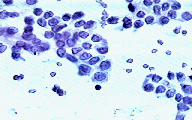
\includegraphics[]{images/fna_nuclei.png}
  \caption{A caption of a FNA sample as seen through a microscope. Image courtesy of Wisconsin University}
  \label{fig:fna_nuclei}
\end{figure}

% Image source: http://webcache.googleusercontent.com/search?q=cache:635J2rrIdWsJ:pages.cs.wisc.edu/~olvi/uwmp/cancer.html+&cd=1&hl=sv&ct=clnk&gl=se


\section{Machine learning}

Here is some very high level text introducing the reader to the concept of machine learning. It end in a way that naturally transitions to explaining different methods.

\subsection{Artificial neural networks}

A artificial neural network (ANN) is a learning model that conceptually consists of a network of nodes and connections. 

\subsection{Decision Trees}

Text here.

\subsection{Naive Bayes}

Text here.

\subsection{Support vector machines}

Text here.

\section{Feature Selection}

A feature is a variable that describes a data instance. A rectangular surface can be considered having two features, length and height. A rectangular volume three features, length, height and depth. More complex data instances such as a gene expression may have up to 60,000 features and such a complex feature space results in a much harder learning process. Thus one often wishes to select a subset of all available to reduce the dimensionality \parencite{guyon2003}.

The benefits of selecting a subset of all available features are manyfold, among other it facilitates data visualisation and data understanding, reduces the measurement and storage requirements and reduces training and utilisation times. In cases with thousands of features like the example with gene expressions it is essential to work with a subset of the data to produce reliable results. \parencite{guyon2003}.


\subsection{Filter methods}

Filter methods are considered as a preprocessing step. That means a filter method evaluate features before data is applied to a learning machine or even before a deciding on a classifier. The evaluation is performed by doing variable ranking by some score such as information gain. The score results in a ranking of the attributes and a subset can be selected in order of the ranking \parencite{guyon2003}.

There are both good and bad aspects of filter methods. The positive concerns that variable ranking makes filter methods very scalable and robust as the calculations only operated on as many variables as there are features and can be performed just once and tested on multiple classifiers making it very computational effective. On the other hand, a subset of features that by their own might be assessed an non informative by their own may in combination provide a lot of information to enable good learning \parencite{guyon2003}.


\subsection{Wrapper methods}

\textbf{ Pawel: Add information on each classifier. At most 1/3 of a page describing their functionality on  vary high level }

Wrapper methods differs a lot from filter methods. While filter methods evaluate the as a preprocessing independent of the classifier, wrapper does the opposite.

Wrappers utilise the learning machine of interest as a black box to score subsets of variable according to their predictive power \parencite{guyon2003}. The issue is as datasets become very large this method might be overly computational intense as finding the optimal subset is considered to be NP-hard \parencite{amaldi1998}.


\section{Related Work}

\textbf{ Pawel: Make subsections where each section coves a specific topic. This can also be extended with almost another full page.}

The application of machine learning onto breast cancer classification is a well studied one. Since machine learning proved valuable empirical results breast cancer datasets have been widely used to assess the performance of a multitude of classification strategies and methods. [Insert ref. to early paper here].

Exhaustive studies for optimal Classifiers has been made as by \parencite{ramos2012} which tested 20,000 classification configurations to evaluated their ability to correctly classify malignant cancer. The achieved a result of 0.996 under the Receiver operating characteristic (ROC) curve.
% Add which method achieved the result above

With a foundation of well performing classifiers studies investigating more fine tuned approaches building upon earlier results were being made. \textcite{akin2011} demonstrated that ensemble learning can be used in CAD to improve the performance of rotation forest classifier. Using three different dataset and 30 classifying algorithms the average accuracy improved on all datasets by nearly 3\%.

\textcite{Abdel-Ilah2017} reported further improvements on ANNs by investigating the optimal number of hidden layers and neurons for a feed forward back propagation network. The highest accuracy acheived was 98\% using 3 hidden layers and 21 neurons with three distinct transfer functions.

\textcite{akay2009} investigated the performance of classification of a SVM with a RBF kernel using feature selection, filtering by F-score. They achieved a classification accuracy of 99.51\% which accordingly was among the highest scores recorded by then (2007).

\textcite{karabulut2012} made a comparative study on the effect of feature selection on classification accuracy and found up to 15.55\% improvement on classification rates. The study used only filter algorithms for feature selection, among those were both information and Chi-square. The study applied the selected features on three classification methods, Naive Bayes, Artificial Neural Network as Multilayer Perceptron, and J48 decision tree classifier on 15 different datasets including WBCD.

Building upon this foundation of work our study seeks to complete the field by providing further investigation of unreported selection methods such as SBS and SFS and review their performance on a combination of classifiers from the previous research presented here.


% --- 3. METHOD CHAPTER ---
\chapter{Method}

\section{Datasets}
\label{sec:Datasets}


\subsection{Wisconsin}

The dataset used in this thesis, Breast Cancer Wisconsin (Diagnostic) dataset, was donated 1995 to UCI  Machine Learning Repository \parencite{dua:2017} by one of its creators, Nick Street. It contains 569 instances with 32 attributes describing the features of breast cancer. Each instance is classified as benign (357) or malignant (212). The 32 attributes describe ten real-value features which are:

% Skip this extended description the dataset?
% \begin{itemize} \itemsep0pt \parskip0pt \parsep0pt
% 	\item \textbf{Radius:} Mean of distances from center to points on the perimeter.
% 	\item \textbf{Texture:} Standard deviation of gray-scale values.
% 	\item \textbf{Smoothness:} Local variation in radius lengths.
%   \item \textbf{Compactness:} perimeter\textsuperscript{2} / area - 1.
%   \item \textbf{Concavity:} Severity of concave portions of the contour.
%   \item \textbf{Concave points:} Number of concave portions of the contour.
%   \item \textbf{Fractal dimension:} Coastline approximation - 1.
%   \item \textbf{Perimeter:} Local variation in radius lengths.
%   \item \textbf{Area}
%   \item \textbf{Symmetry}
% \end{itemize}


\subsection{Royal Hallamshire Hospital}

Fine needle aspirates of breast lumps (FNAB) was collected from 692 patients at Royal Hallamshire Hospital, Sheffield, during 1992 - 1993. The FNABs 10 features of the FNABs was marked as present or non present. These features along with the patients's age defines the attributes of the dataset. In addition, the final outcome of benign disease or malignancy was confirmed by open biopsy where this result was available.

\subsection{MIAS database}

Mias database contain results from 119 data points with 5 features: Character of background tissue, Class of abnormality, X coordinate of centre of abnormality, Y coordinate of centre of abnormality, Approximate radius (in pixels). The features was extracted from 1024x1024 pixel images.

% Skip RNA dataset
% \subsection{U.S. National Centre for Biotechnology Information}
%
% The data contains information on 1919 microRNAs in 122 different cases.

\subsection{Erlangen-Nuremberg}

Dataset collected from a Breast Imaging-Reporting and Data System (BI-RADS) at the Institute of Radiology of the University Erlangen-Nuremberg between 2003 and 2006. It contains three features assessed as a discrete value from a double-review by physicians along with the patients' age.

% Table with information on Datasets
\medskip
\begin{table}[ht!]
\begin{adjustwidth}{-5.in}{-5.in}
\begin{center}
   \begin{tabular}{l*{4}{l}}
   \hline
   Dataset         &
   \# examples  &
   \# features  &
   Ratio (B/M)     &
   Type            \\
   \hline
   Wisconsin (WBCD)						 &
   569                         &
   32                          &
   357/212                     &
   Continous                   \\
   Royal Hallamshire Hospital (RHH)  &
   692                         &
   11                          &
   457/235                     &
   Binary                      \\
   Erlangen-Nuremberg (EN)     &
   961                         &
   5                           &
   516/445                     &
   Discrete                    \\
   MIAS         							 &
   119                         &
   5                           &
   68/51                     	 &
   Discrete                    \\
  \hline
  \end{tabular}
  \caption{Datasets}
  \label{table:datasets_info}
\end{center}
\end{adjustwidth}
\end{table}


\section{Implementation}

\subsection{Classifiers}
All classifiers was implemented using Sklearn's library. \textbf{[insert: reference]} All setting of each classifier is presented in table \textbf{[insert: table reference]}.

\subsection{Feature selection}

We've used sklearn for filtering methods and mlextend for the Wrapper methods...

\section{Evaluation}

What methods are implemented to measure the results, are we using mean, standard deviation, f1 score, anova, how many times do we run etc...

% Pawel: Describe all configurations of classifiers and feature selection methods, discuss how you choose parameters, train them (on what data with what algorithms etc.)


% --- 4. RESULTS AND ANALYSIS CHAPTER ---
\chapter{Results and analysis}

We performed classification with four different classifiers on four different datasets. In each dataset-classifier combination we measured classification accuracy when applying four different feature selection (FS) methods. The aim is to investigate the impact of feature selection, and the interaction between different classifiers and FS-methods. To build a basis for comparisons, classification accuracy was measured without FS too.

\section{Variation among factors of experiments}
\label{Variation_among_factors}

Before analyzing the results we consider potential interactions between different factors involved in the experiment, these are:

\begin{enumerate}
  \item Datasets
  \item Machine Learning classifiers
  \item Feature selection methods
\end{enumerate}

Having four of each factor, there are 64 distinct combinations. We are particular interested in two of the interactions, Datasets:FS-methods and Classifiers:FS-methods.

\subsection{Datasets with larger dimensionality achieves better classification accuracy}

Studying the interaction between datasets and FS-methods, we regarded these factors as independent variables (IVs). Each IV combination is represented by four values, the best accuracy achieved with current FS-method by each of the four classifiers.

Two-way analysis of variance (ANOVA) is performed on the IVs. The results are found in \ref{table:anova_values_data} and suggests three conclusions:

% ANOVA computations, dataset-fs
\begin{table}[ht]
  \begin{center}
  \begin{tabular}{l|r|r|r|r|r|r|}
  \cline{2-7}
  & $RSS$ & $df$ & $F$ & $P(>F)$ & $\eta^2$ & $\omega^2$ \\ \cline{1-7}
  \multicolumn{1}{ |l| }{\textbf{Dataset}}
  & 0.7383 &  3.0 & 15.939 & 2.5241e-07 & 0.4757 & 0.4415 \\
  \cline{1-7}
  \multicolumn{1}{ |l| }{\textbf{Method}}
  & 0.0099 &  3.0 & 0.2137 & 8.8645e-01 & 0.0064 & -0.0232 \\
  \cline{1-7}
  \multicolumn{1}{ |l| }{\textbf{Dataset:Method}}
  & 0.0627 &  9.0 & 0.4514 & 8.9938e-01 & 0.0404 & -0.0486 \\
  \cline{1-7}
  \multicolumn{1}{ |l| }{\textbf{Residual}}
  & 0.7412 &  48.0 \\ \cline{1-3}
  \end{tabular}
  \caption{ANOVA values of accuracy in relation to dataset, method and the interaction of datasets and methods.}
  \label{table:anova_values_data}
  \end{center}
\end{table}


First, the significance of Dataset allows to conclude a dependency between accuracies and datasets is present. This is to be expected because different datasets provide varying basis for prediction. However, as all accuracies used in the test was obtained by feature selection this test gives no information on whether the correlation lies among the datasets themselves of the application of feature selection.

Secondly, absent significance of Method conclude we can not reject that there is no correlation between FS-method and accuracy.

Thirdly, no significance of Dataset:Method indicates we can not reliably conclude that the interaction between datasets and methods has a correlation with achieved accuracy.

Visualizing the values used in the ANOVA test we can spot the found correlation between datasets and accuracy \ref{fig:comp_acc_datasets}. The correlation appears positive in respect to number of attributes suggesting either feature selection has a larger impact on classification accuracy when data has a higher dimensionality or higher dimensioned datasets on their own lead to better accuracy.

\begin{figure*}[ht]
  \centering
    \begin{subfigure}[b]{0.475\textwidth}
        \centering
        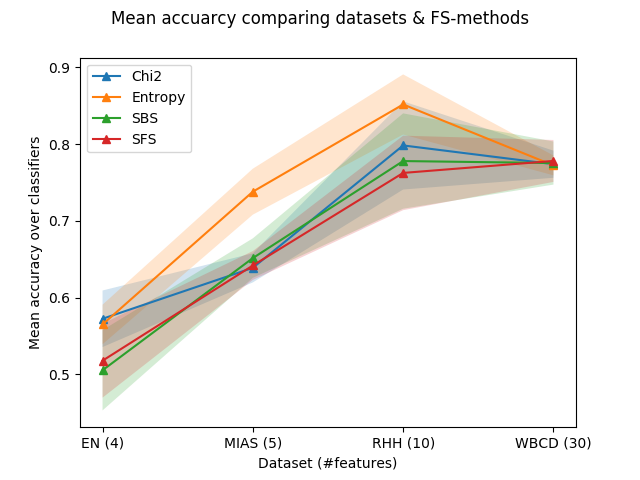
\includegraphics[width=\textwidth]{../plots_with_std_fill/comp_acc_datasets.png}
        \caption[]%
        {{\small Datasets and accuracy displays evident correlation independently of applied FS method.}}
        \label{fig:comp_acc_datasets}
    \end{subfigure}
  \hfill
    \begin{subfigure}[b]{0.475\textwidth}
        \centering
        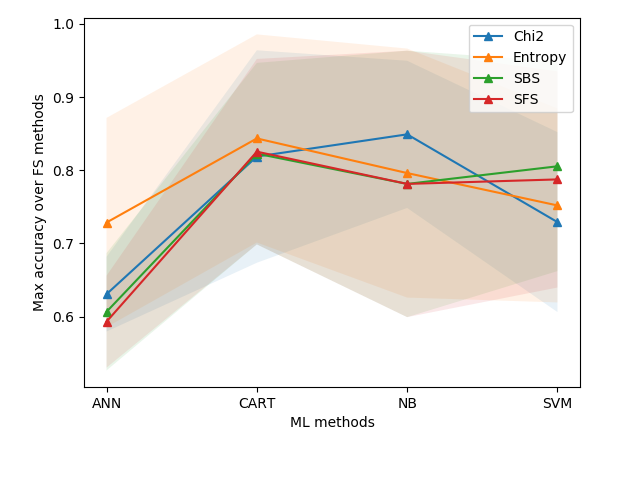
\includegraphics[width=\textwidth]{../plots_with_std_fill/comp_classif_datasets.png}
        \caption[]%
        {{\small Some correlation between different classifiers and FS-methods is evident.}}
        \label{fig:comp_classif_datasets}
    \end{subfigure}
  \caption[]
  {\small Good caption goes here.}
  \label{fig:anova_plots}
\end{figure*}


\subsection{FS-methods are classifier dependent}
\label{sec:fs_methods_classifiers}

To investigate the effect of feature selection on different classifiers we performed two-way ANOVA. The values constitutes of each accuracy achieved of all distinct classifier and FS-method on all datasets. The values are presented in \ref{table:anova_values_classif}.

\begin{table}[ht]
  \begin{center}
  \begin{tabular}{l|r|r|r|r|r|r|}
  \cline{2-7}
  & $RSS$ & $df$ & $F$ & $P(>F)$ & $\eta^2$ & $\omega^2$ \\ \cline{1-7}
  \multicolumn{1}{ |l| }{\textbf{Classifier}}
  & 0.3336 &  3.0 & 16.491 & 1.6860e-07 & 0.2149 & 0.2010 \\
  \cline{1-7}
  \multicolumn{1}{ |l| }{\textbf{Method}}
  & 0.7383 &  3.0 & 36.495 & 1.9503e-12 & 0.4757 & 0.4607 \\
  \cline{1-7}
  \multicolumn{1}{ |l| }{\textbf{Classifier*Method}}
  & 0.1565 &  9.0 & 2.5783 & 1.6490e-02 & 0.1008 & 0.0614 \\
  \cline{1-7}
  \multicolumn{1}{ |l| }{\textbf{Residual}}
  & 0.3237 &  48.0 \\ \cline{1-3}
  \end{tabular}
  \caption{Set caption.}
  \label{table:anova_values_classif}
  \end{center}
\end{table}


The significance of both Classifier and Method concludes they independently effect what accuracy is achieved. Their interaction, Classifier:Method is significant too and allows to reason there is a dependency between accuracy and the interaction between classifiers and methods. Plotting the values used in the test visualizes this correlation \ref{fig:comp_classif_datasets}.

To further analyze the interaction we performed post-hoc analysis by Tukey's test \parencite{Haynes2013}. The significant results \ref{table:Tukey_values} show the difference among the groups lies mainly in which classifier is used. Only in the case of SVM difference in classification rate is seen with same classifier and different classification methods. In these instances wrapper methods performed 21\% and 33\% better than chi2.

To conclude these results, they suggests one primarily has to carefully select the classifier to use for classification. When choosing SVM the choice of feature selection has greatest impact.


\section{Classification improvements}

After performing classification with and without FS-methods, all results of each classifier was collected. Results are presented in tables for ANN \ref{table:ANN}, CART \ref{table:CART}, NB \ref{table:NB} and SVM \ref{table:SVM} where the highest achieved accuracy is highlighted in bold format. The improvement is measures in gain, it is the ratio between best achieved FS accuracy and full dataset accuracy. From this we can conclude that classification accuracy is equal or improved for all classifiers on all datasets tested in our scope by use of \textit{some} feature selection method. The only exception is the Mias dataset with Decision tree \ref{table:CART}, it performed worse with feature selection.

However, majority of the classifiers has some FS-method that achieved lower accuracy compared to full dataset. Again this is viewed in tables \ref{table:ANN}, \ref{table:CART}, \ref{table:NB} and \ref{table:SVM}. In 11 of 16 instances at least one FS-method performed worse. This is in line with our findings that FS-method is classifier dependent suggesting one have to select the combination of classifier and FS-method with care.

% --- Tables ---
\begin{table}[h]
  \centering
  \begin{tabular}{|l|l|l|l|l|l}
\cline{1-5}
        \textbf{ANN} & MIAS              & EN                & RHH               & WBCD      &         \\
\cline{1-5}
Chi2    & 0.58 & 0.59 & 0.64 & 0.71 \\
Entropy & 0.56 & \textbf{0.84} & \textbf{0.90} & 0.62 \\
SBS     & 0.54 & 0.55 & 0.59 & \textbf{0.74} \\
SFS     & \textbf{0.59} & 0.51 & 0.59 & 0.68 \\
Full    & 0.57 & 0.68 & 0.60 & 0.53 \\
\cline{1-5}
Gain    & 0.04 & 0.24 & 0.51 & 0.41 & 1.2 \\
\cline{1-5}
\end{tabular}

  \caption[]%
  {{\small Classification accuracy achieved by ANN. Accuracy improved on all datasets by the use of some feature selection method. Rows represent feature selection method, columns represent dataset, bold font indicates the highest value.}}
  \label{table:ANN}
\end{table}

\begin{table}[h]
  \centering
  \begin{tabular}{|l|l|l|l|l|l}
\cline{1-5}
        \textbf{CART} & MIAS              & EN                & RHH               & WBCD      &         \\
\cline{1-5}
Chi2    & 0.70           & 0.69           & 0.90           & \textbf{0.97}  &         \\
Entropy & 0.53           & \textbf{0.83}  & 0.91           & 0.96           &         \\
SBS     & 0.63           & 0.67           & 0.91           & 0.95           &         \\
SFS     & 0.67           & 0.67           & \textbf{0.92}  & \textbf{0.97}  &         \\
Full    & \textbf{0.77}  & 0.69           & 0.90           & 0.94           &         \\
\cline{1-5}
\cline{1-5}
Gain    & -0.09           & 0.21           & 0.03           & 0.03           & 0.18 \\
\cline{1-5}
\end{tabular}
 \\
  \caption[]%
  {{\small All datasets except MIAS benefited in classification accuracy from feature selection using CART Decision Tree classifier. Rows represent feature selection method, columns represent dataset, bold font indicates the highest value.}}
  \label{table:CART}
\end{table}

\begin{table}[h]
  \centering
  \begin{tabular}{|l|l|l|l|l|l}
\cline{1-5}
        & MIAS              & EN                & RHH               & WBCD      &         \\
\cline{1-5}
Chi2    & \textbf{0.77}  & \textbf{0.74}  & \textbf{0.94}  & 0.96           &         \\
Entropy & \textbf{0.77}  & 0.55           & 0.91           & 0.97           &         \\
SBS     & 0.43           & 0.71           & 0.91           & \textbf{0.97}  &         \\
SFS     & 0.43           & 0.71           & 0.91           & \textbf{0.97}  &         \\
Full    & \textbf{0.77}  & 0.66           & \textbf{0.94}  & 0.96           &         \\
\cline{1-5}
\cline{1-5}
Gain    & 0                 & 0.12           & 0                 & 0.01           & 0.14 \\
\cline{1-5}
\end{tabular}
 \\
  \caption[]%
  {{\small Na\"ive Bayes sees improvement or equivalent accuracy by feature selection on every dataset. Rows represent feature selection method, columns represent dataset, bold font indicates the highest value.}}
  \label{table:NB}
\end{table}

\begin{table}[h]
  \centering
  \begin{tabular}{|l|l|l|l|l|l}
\cline{1-5}
        \textbf{SVM} & MIAS              & EN                & RHH               & WBCD      &         \\
\cline{1-5}
Chi2    & \textbf{0.57}  & 0.73           & 0.90           & 0.63           &         \\
Entropy & 0.33           & \textbf{0.83}  & \textbf{0.91}  & 0.63           &         \\
SBS     & 0.53           & 0.68           & 0.88           & \textbf{0.93}  &         \\
SFS     & 0.53           & 0.68           & 0.88           & \textbf{0.93}  &         \\
Full    & \textbf{0.57}  & 0.73           & 0.90           & 0.61           &         \\
\cline{1-5}
\cline{1-5}
Gain    & 0                 & 0.14           & 0.02           & 0.51           & 0.68 \\
\cline{1-5}
\end{tabular}
 \\
  \caption[]%
  {{\small Classification accuracy achieved by SVM. Accuracy was improved or equivalent on every dataset with use of feature selection. Rows represent feature selection method, columns represent dataset, bold font indicates the highest value.}}
  \label{table:SVM}
\end{table}
% ---/Tables ---

\subsection{Improvement is significant}

To ensure the suggestion that application of some FS-method improves classification accuracy t-test was performed. The t-test values constitutes of the accuracies achieved without feature selection as one distribution. The other are the best accuracies achieved with feature selection. The t-test values are summarized in \ref{table:t_test_values}.

\begin{table}[h]
  \centering
  \begin{table}[htb]

    \noindent\makebox[\textwidth]{%

      \begin{subtable}{0.65\linewidth}
        \centering
          \begin{tabular}{|l|l|l|l|l|l}
          \cline{1-5}
          \textbf{FS}      & MIAS           & EN             & RHH            & WBCD           &         \\
          \cline{1-5}
          ANN     & 0.63           & 0.83           & 0.90           & 0.73           &         \\
          CART    & 0.67           & 0.83           & 0.92           & 0.97           &         \\
          NB      & 0.77           & 0.74           & 0.94           & 0.97           &         \\
          SFS     & 0.57           & 0.83           & 0.91           & 0.93           &         \\
          \cline{1-5}
          \end{tabular}
          \caption[]
          \small{}
      \end{subtable}%
      \begin{subtable}{0.65\linewidth}
        \centering
          \begin{tabular}{|l|l|l|l|l|l}
          \cline{1-5}
          \textbf{Full}    & MIAS           & EN             & RHH            & WBCD           &         \\
          \cline{1-5}
          ANN     & 0.60           & 0.53           & 0.57           & 0.64           &         \\
          CART    & 0.77           & 0.69           & 0.90           & 0.94           &         \\
          NB      & 0.77           & 0.66           & 0.94           & 0.96           &         \\
          SFS     & 0.57           & 0.73           & 0.90           & 0.61           &         \\
          \cline{1-5}
          \end{tabular}
          \caption[]
          \small{}
      \end{subtable}
    }

    \caption[]%
    {\small
      (a) The highest accuracy achieved by any FS-method on all classifier-dataset combinations. (b) corresponding accuracies achieved without any feature selection on Full dataset. T-test comparing the distributions results in significantly higher results by classification with feature selection.}
    \label{table:t_test_values}

\end{table}
 \\
  \caption[]%
  {{\small The highest accuracy achieved by any FS-method on all classifier-dataset combinations and corresponding accuracies achieved without any feature selection (Full). T-test comparing the distributions results in significantly higher results by classification with feature selection.}}
  \label{table:t_test_values}
\end{table}

Performing the t-test resulting P-value was 0.077. This allows us to reject the null hypothesis that the distributions are equal with a confidence level of 90\%. Thus, improvement of classification accuracy by feature selection is statistically significant.

\subsection{Differences among classifiers}

As addressed in section \ref{Variation_among_factors} classifiers behave differently depending on FS-method and datasets.
In order to compare classification improvement among different FS-methods and datasets \textbf{Gain} is computed. Gain measures the improvement of FS as the ratio between best achieved FS accuracy and full dataset accuracy. The accumulated gain for each classifier is presented in \ref{table:gain_comparison}. Below these results and differences are analyzed in further detail with respect to each classifier.

\begin{table}[hp]
  \begin{tabular}{|l|l|l|l|}
\hline
Ranking  & Classifier                & Accumulated gain  & Average gain\\
\hline
1        & Artificial Neural Network & 1.34   & 34\%        \\
2        & Support Vector Machine    & 0.68  & 17\%       \\
3        & Decision Tree             & 0.18   & 5\%         \\
4        & Naïve Bayes               & 0.14   & 4\%         \\
\hline
\end{tabular}

  \caption[]%
  {{\small Ranking of which classifiers gained most accuracy when comparing feature selection to full dataset.}}
  \label{table:gain_comparison}
\end{table}

\subsubsection{Artificial Neural Network}

Looking at the table \ref{table:gain_comparison} the accumulated gain was 1.34 which was the highest among all classifiers. However, ANN consistently performs the worst of all classifiers in terms of accuracy. The ANN also provides the least consistent results with strong fluctuations in the results and wide standard deviation margins. Such fluctuations may suggest issues regarding convergence. These characteristics are evident in plot \ref{fig:WBCD_chi2} showcasing the accuracy by each FS-method as a function of number of attributes..

\subsubsection{Support Vector Machine}

The SVM behaves very differently in respect to each dataset. Improvements are seen with a larger subset of attributes in the EN and MIAS dataset as seen in \ref{fig:EN_chi2} and \ref{fig:MIAS_sfs}. A negative trend on accuracy is observed on the WBCD datasets which might indicate an issue with dimensionality. In \ref{fig:RHH_sbs} an improved accuracy is evident with maximal accuracy achieved on a subset suggesting a positive effect of feature selection.

\subsubsection{Decision Tree}

The decision tree shows consistent performance generally increasing performance with an increased amount of features. Although in cases like plot \ref{fig:WBCD_chi2} and \ref{fig:MIAS_sbs} best accuracy is achieved with a subset of features displaying evident benefits of feature selection.

\subsubsection{Naïve Bayes}

Naive Bayes had the least accumulated gain from feature selection as seen in table \ref{table:gain_comparison}. The largest improvement was seen in plot \ref{fig:EN_chi2} using 2 of 4 available attributes. In plots \ref{fig:WBCD_entropy} and \ref{fig:RHH_entropy} the accuracy sees little to no improvement when increasing the number of attributes.

\subsection{Combined plots of mean accuracy}
\begin{figure*}[htp]
  \centering
  \begin{subfigure}[b]{0.475\textwidth}
      \centering
      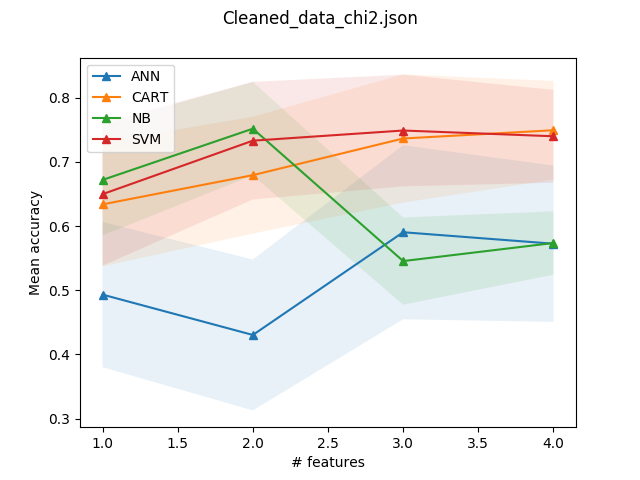
\includegraphics[width=\textwidth]{../plots_with_std_fill/Cleaned_data_chi2_combined.png}
      \caption[]%
      {{\small}}
      \label{fig:EN_chi2}
  \end{subfigure}
  \hfill
  \begin{subfigure}[b]{0.475\textwidth}
      \centering
      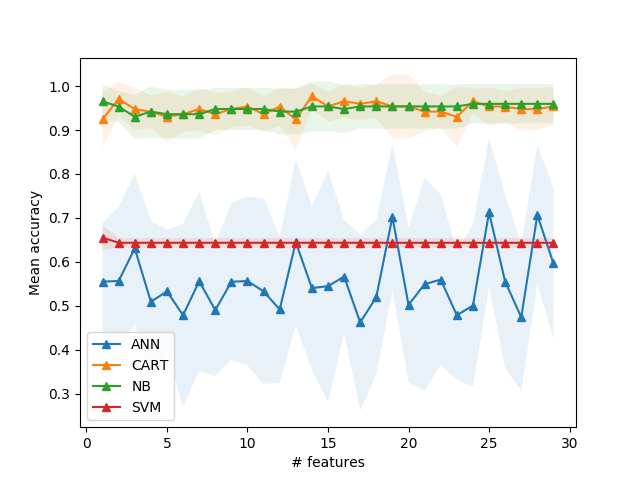
\includegraphics[width=\textwidth]{../plots_with_std_fill/data_FNA_chi2_combined.png}
      \caption[]%
      {{\small}}
      \label{fig:WBCD_chi2}
  \end{subfigure}
  \vskip\baselineskip
  \begin{subfigure}[b]{0.475\textwidth}
      \centering
      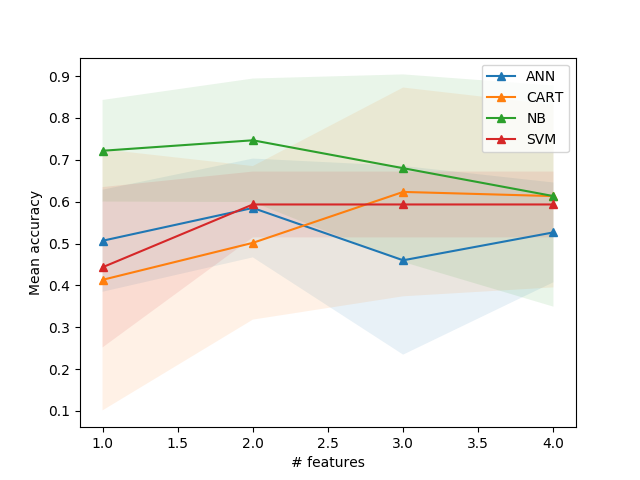
\includegraphics[width=\textwidth]{../plots_with_std_fill/Data_mias_chi2_combined.png}
      \caption[]%
      {{\small}}
      \label{fig:MIAS_chi2}
  \end{subfigure}
  \quad
  \begin{subfigure}[b]{0.475\textwidth}
      \centering
      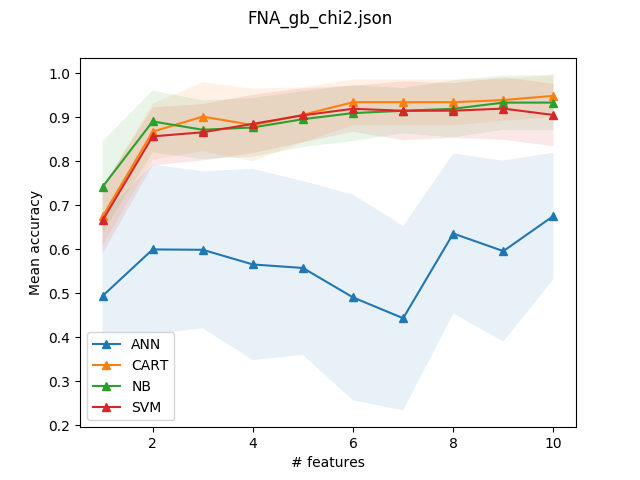
\includegraphics[width=\textwidth]{../plots_with_std_fill/FNA_gb_chi2_combined.png}
      \caption[]%
      {{\small}}
      \label{fig:RHH_chi2}
  \end{subfigure}
  \caption[]
  {\small a: Dataset EN using Chi2, b: Dataset WBCD using Chi2, c:  Dataset MIAS using Chi2, d: Dataset RHH using Chi2.  Combined plots of all datasets comparing each classifier when using chi2 for feature selection.}
  \label{fig:plots_chi2}
\end{figure*}

\begin{figure*}[htp]
  \centering
  \begin{subfigure}[b]{0.475\textwidth}
      \centering
      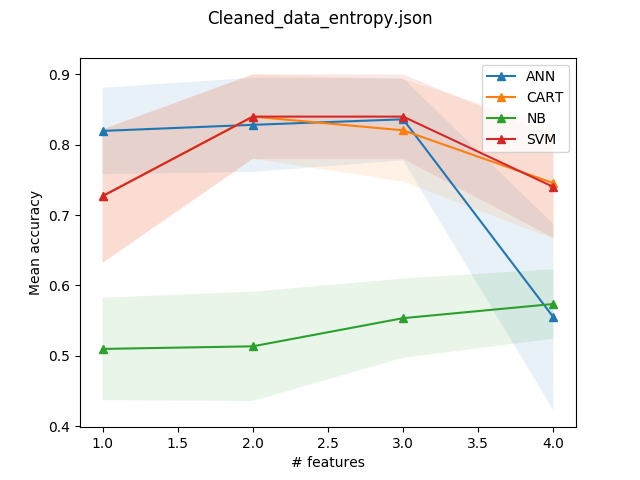
\includegraphics[width=\textwidth]{../plots_with_std_fill/Cleaned_data_entropy_combined.png}
      \caption[Network2]%
      {{\small }}
      \label{fig:EN_entropy}
  \end{subfigure}
  \hfill
  \begin{subfigure}[b]{0.475\textwidth}
      \centering
      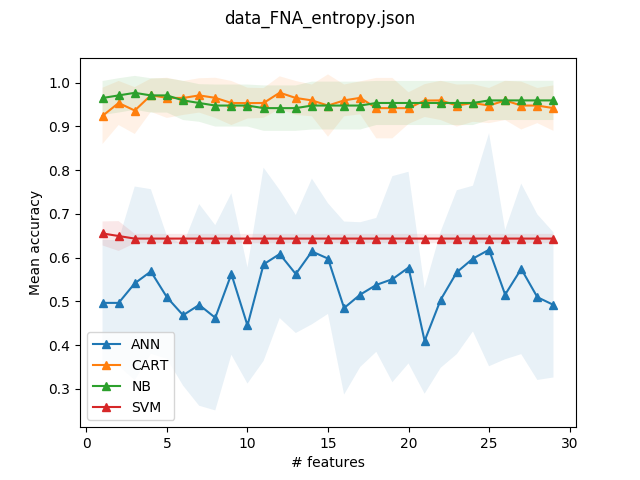
\includegraphics[width=\textwidth]{../plots_with_std_fill/data_FNA_entropy_combined.png}
      \caption[]%
      {{\small}}
      \label{fig:WBCD_entropy}
  \end{subfigure}
  \vskip\baselineskip
  \begin{subfigure}[b]{0.475\textwidth}
      \centering
      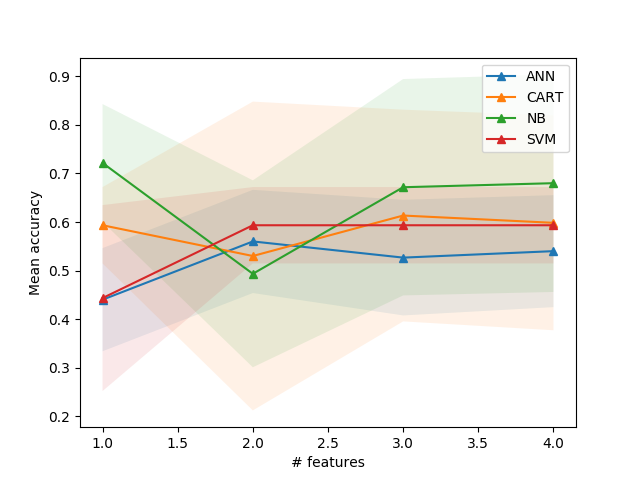
\includegraphics[width=\textwidth]{../plots_with_std_fill/Data_mias_entropy_combined.png}
      \caption[]%
      {{\small }}
      \label{fig:MIAS_entropy}
  \end{subfigure}
  \quad
  \begin{subfigure}[b]{0.475\textwidth}
      \centering
      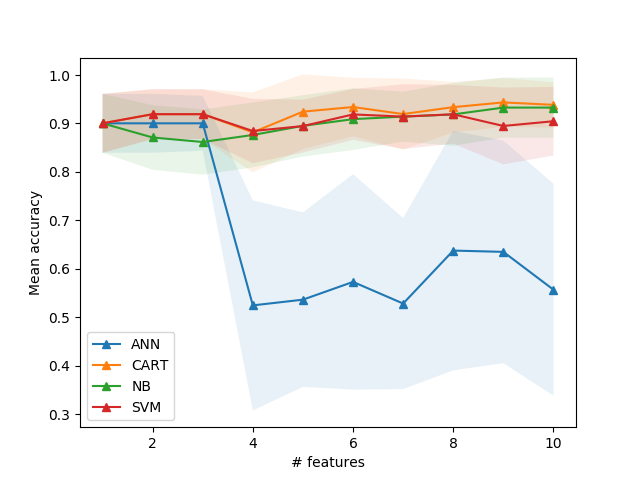
\includegraphics[width=\textwidth]{../plots_with_std_fill/FNA_gb_entropy_combined.png}
      \caption[]%
      {{\small }}
      \label{fig:RHH_entropy}
  \end{subfigure}
  \caption[]
  {{\small a: Dataset EN using Entropy, b: Dataset WBCD using Entropy, c: Dataset MIAS using Entropy, d: Dataset RHH using Entropy. Combined plots of all datasets comparing each classifier when using Entropy for feature selection.}}
  \label{fig:plots_entropy}
\end{figure*}

\begin{figure*}[htp]
  \centering
  \begin{subfigure}[b]{0.475\textwidth}
      \centering
      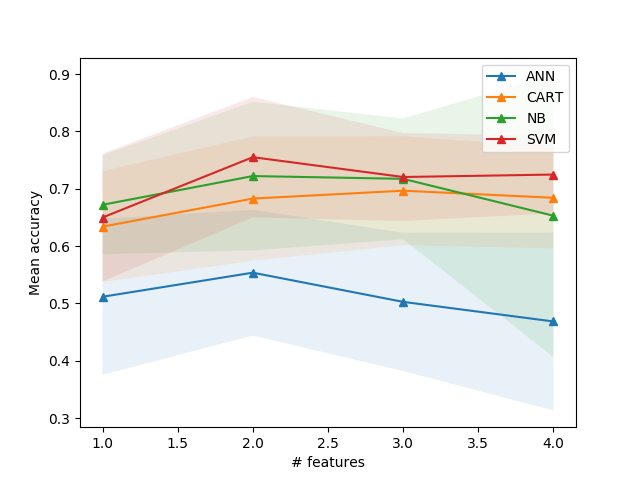
\includegraphics[width=\textwidth]{../plots_with_std_fill/Cleaned_data_sb_combined.png}
      \caption[]%
      {{\small}}
      \label{fig:EN_sbs}
  \end{subfigure}
  \hfill
  \begin{subfigure}[b]{0.475\textwidth}
      \centering
      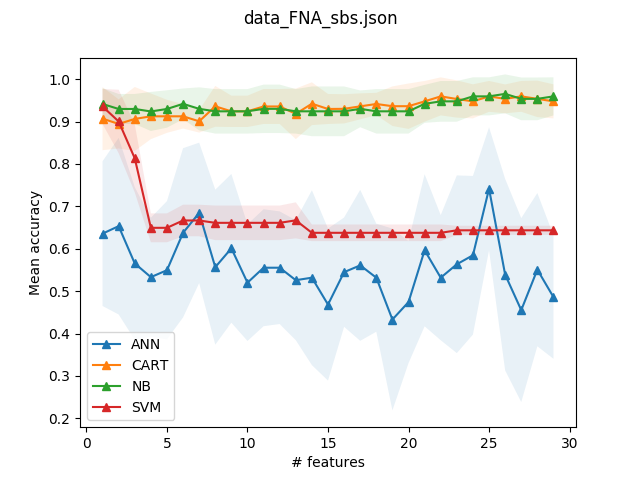
\includegraphics[width=\textwidth]{../plots_with_std_fill/data_FNA_sb_combined.png}
      \caption[]%
      {{\small}}
      \label{fig:WBCD_sbs}
  \end{subfigure}
  \vskip\baselineskip
  \begin{subfigure}[b]{0.475\textwidth}
      \centering
      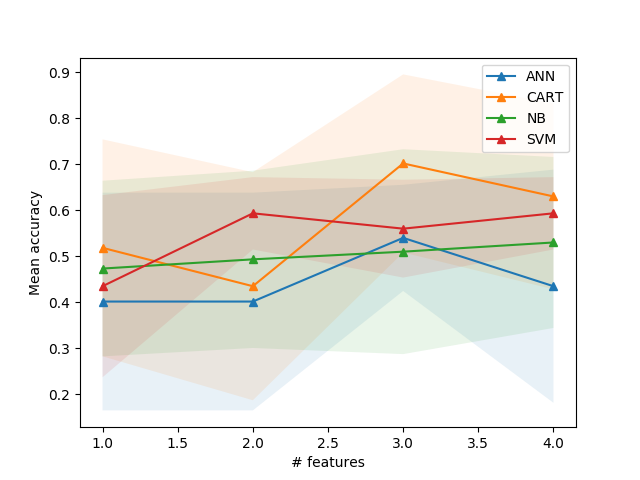
\includegraphics[width=\textwidth]{../plots_with_std_fill/Data_mias_sb_combined.png}
      \caption[]%
      {{\small}}
      \label{fig:MIAS_sbs}
  \end{subfigure}
  \quad
  \begin{subfigure}[b]{0.475\textwidth}
      \centering
      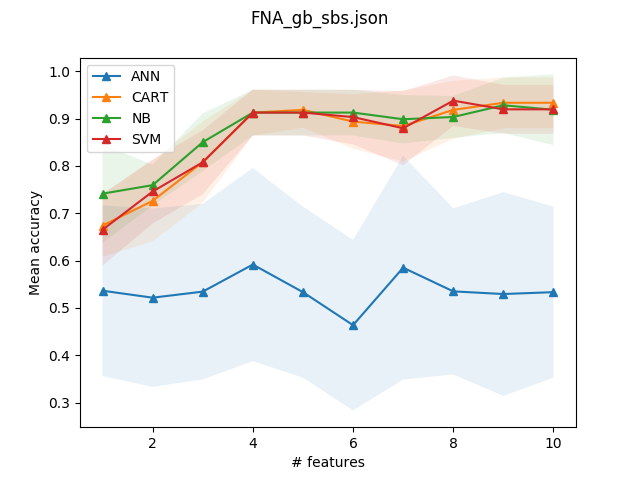
\includegraphics[width=\textwidth]{../plots_with_std_fill/FNA_gb_sb_combined.png}
      \caption[]%
      {{\small}}
      \label{fig:RHH_sbs}
  \end{subfigure}
  \caption[]
  {{\small (a) Dataset EN using SBS. (b) Dataset WBCD using SBS. (c) Dataset MIAS using SBS. (d) Dataset RHH using SBS. Combined plots of all datasets comparing each classifier when using SBS for feature selection.}}
  \label{fig:plots_sbs}
\end{figure*}

\begin{figure*}[htbp!]
  \centering
  \begin{subfigure}[b]{0.475\textwidth}
      \centering
      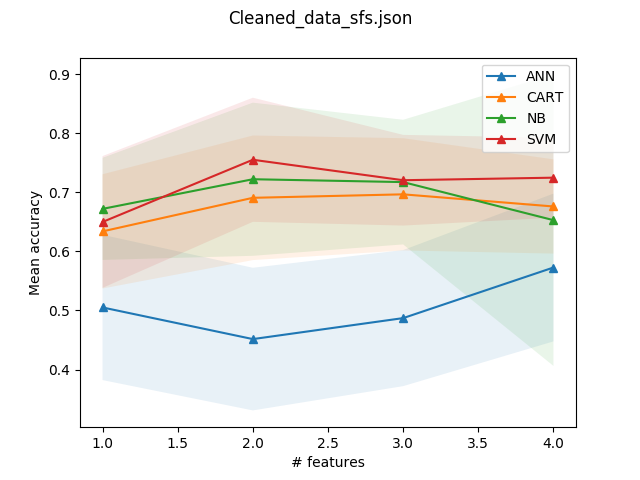
\includegraphics[width=\textwidth]{../plots_with_std_fill/Cleaned_data_sf_combined.png}
      \caption[]%
      {{\small Dataset EN using SFS}}
      \label{fig:EN_sfs}
  \end{subfigure}
  \hfill
  \begin{subfigure}[b]{0.475\textwidth}
      \centering
      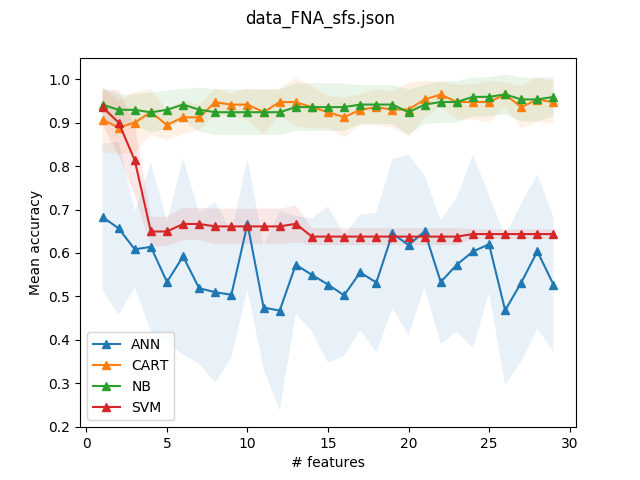
\includegraphics[width=\textwidth]{../plots_with_std_fill/data_FNA_sf_combined.png}
      \caption[]%
      {{\small Dataset WBCD using SFS}}
      \label{fig:WBCD_sfs}
  \end{subfigure}
  \vskip\baselineskip
  \begin{subfigure}[b]{0.475\textwidth}
      \centering
      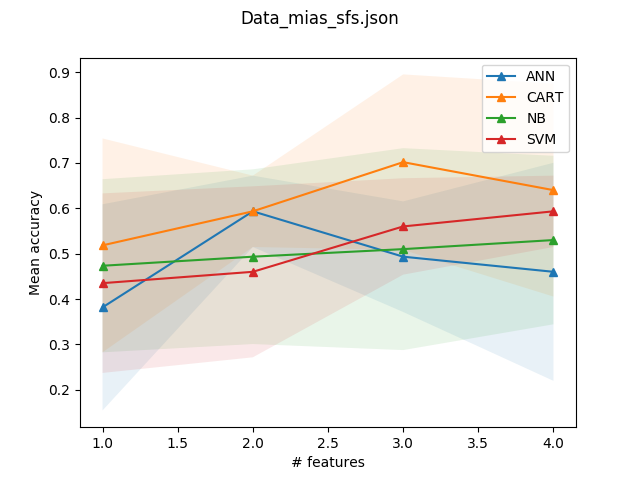
\includegraphics[width=\textwidth]{../plots_with_std_fill/Data_mias_sf_combined.png}
      \caption[]%
      {{\small Dataset MIAS using SFS}}
      \label{fig:MIAS_sfs}
  \end{subfigure}
  \quad
  \begin{subfigure}[b]{0.475\textwidth}
      \centering
      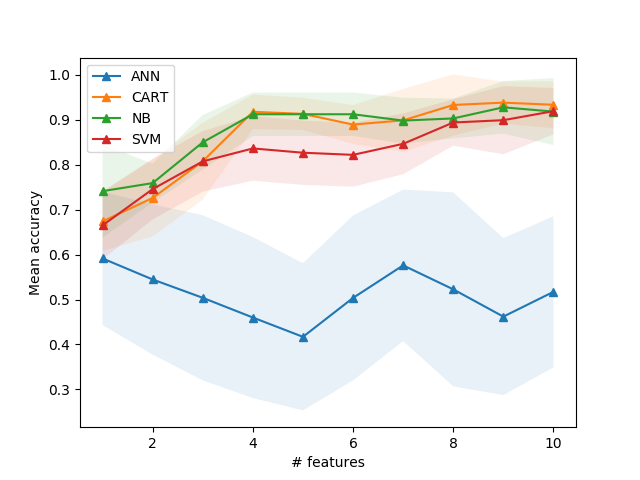
\includegraphics[width=\textwidth]{../plots_with_std_fill/FNA_gb_sf_combined.png}
      \caption[]%
      {{\small Dataset RHH using SFS}}
      \label{fig:RHH_sfs}
  \end{subfigure}
  \caption[]
  {{\small Combined plots of all datasets comparing each classifier when using SFS for feature selection.}}
  \label{fig:plots_sfs}
\end{figure*}



\section{Computation time}

\textbf{Under construction, profiling not run yet.}

Profiling the execution of running all experiments X\% of CPU-time was allocated to the Wrapper algorithms. As mentioned a finding the best possible subset of features is considered a NP-hard problem meaning a solution can not be found in polynomial time. This clearly suggest favouring filtering methods when choosing a feature selection method having limited computational resources.

\section{Source of errors}
\label{sec:source_of_errors}

There are two main factor that may risk propagate error into the results, libraries and datasets.

The libraries provide all functionality of the classifiers, filter selection methods and analysis tools. A major part of the implementation therefore constitutes of these libraries. A implementation built upon faulty methods can not provide any trustworthy results. The Scikit library \parencite{scikit-learn} is well renowned and widely used in both industry and research thus inspire confidence in its robustness. The mlxtend library is used for SBS and SFS methods and is still a open source with less coverage than Scikit \parencite{mlextend}. Still it has a active community and many release versions indicating it's well managed.

Because we use a multitude of datasets their differences may influence our results in a way that invalidates our findings. \textcite{c201416} claim that feature selection methods can only be compared on the same dataset. However our comparisons do not regard the performance of specific FS-methods but their impact at large. Also, these interactions is addressed in \ref{Variation_among_factors}.

Due to varying number of examples of the datasets where some are rather small, evaluation by kFold may infer very small test batches and lead to skewed results. The impact may be enlarged considering our classification is binary. This influence is minimized by using stratified kFold but as no check of distribution of classes in test batches was made this might be a source of error.


% --- 5. DISCUSSION ---
\chapter{Discussion}

\section{Influence of feature selection}

Feature selection is valuable strategy when it comes to classification of breast cancer. As stated in the results all instances but one provided equally good or improved accuracy on the dataset with feature selection compared to using the full dataset. Even in cases where results are equally good feature selection still provide benefits to the process. The benefits consists of potentially lessened effort collecting and processing less attributes at data collection. As stated by \textcite{martei2018} there is a large demand of a more streamlined and efficient process when it comes to breast caner classification, feature selection may offer such a tool.

Choosing the correct combination of classifier and FS-method is essential to produce good results. While some feature selection method nearly always outperform the classifier with the full dataset it does not apply to all FS methods. As filter methods proved computationally fast in comparison to wrappers as as well as better performing, suitable classifiers can be investigated efficiently to find a good subset of features. If wrapper methods are to be used there may be a large benefit in constructing a search approach for the NP-hard part of the problem instead of evaluating the full search space.

As mentioned in source of errors \ref{sec:source_of_errors} using default classifiers might cause the fluctuation and wide variance in the results. A classifier with $n$ attributes might need very different parameters than the same classifier with $n + 1$ parameters to achieve optimal performance. This raises an important question: should a high performing classifier and FS-method be found first then optimised by tuning or it it the other way around?


\section{Limitations}

Due to the limited amount of breast cancer datasets found and utilised in the study its difficult to confidently draw conclusions regarding all breast cancer classification at large.

Limited resources has also resulted in a reduced subset of FS-methods studied. While having two methods of each FS-family, filters and wrappers, there are many more which may have produced different results than we have achieved.


\section{Further research}

Further investigation of a methodology of finding the best possible classifier and FS-method.

More recent strategies of diagnosing breast cancer involves sampling microRNA from patients. Other diseases have been diagnosed with microRNA suggesting promising results of the method. As a sample of microRNA contains around 2 000 features selection may offer a huge benefit.


\section{Ethical aspects}

The data used in this report origin from patients that may be experience discomfort during mammographies, FNA sampling or with other method was used when collecting the data. The data also holds sensitive information ruling the patients future health.

While circumstances of a patient can be very unpleasant such test is a tool to diagnose the patient and potentially discover cancer in time to take necessary action to improve patients' health. Data is to our knowledge never collected without a patients consent and carries no information that can allows identification.

\section{Sustainability}

Under construction...


% --- 6. CONCLUSION ---
\chapter{Conclusion}

I guess this will be the last thing we write



% --- BIBLIOGRAPHY AND APPENDIX ---

\printbibliography[heading=bibintoc] % Print the bibliography (and make it appear in the table of contents)

\appendix
\chapter{Unnecessary Appended Material}

\end{document}
